\section{Scenarios}\label{sec:scenarios}
Illustrate how your architecture fulfills the most important data flows.
As a rule of thumb, focus on the scenario of the domain description.
Describe the scenario in terms of architectural components using UML Sequence
diagrams and further explain the most important interactions in text.
Illustrating the scenarios serves as a quick validation of the completeness of
your architecture.
If you notice at this point that for some reason, certain functionality or
qualities are not addressed sufficiently in your architecture, it suffices to
document this, together with a rationale of why this is the case according to
you.
You do not have to further refine you architecture at this point.

\subsection{Scenario 1}
Shortly describe the scenario shown in this subsection.
Show the complete scenario using one or more sequence diagrams.

\begin{figure}[!htp]
    \centering
    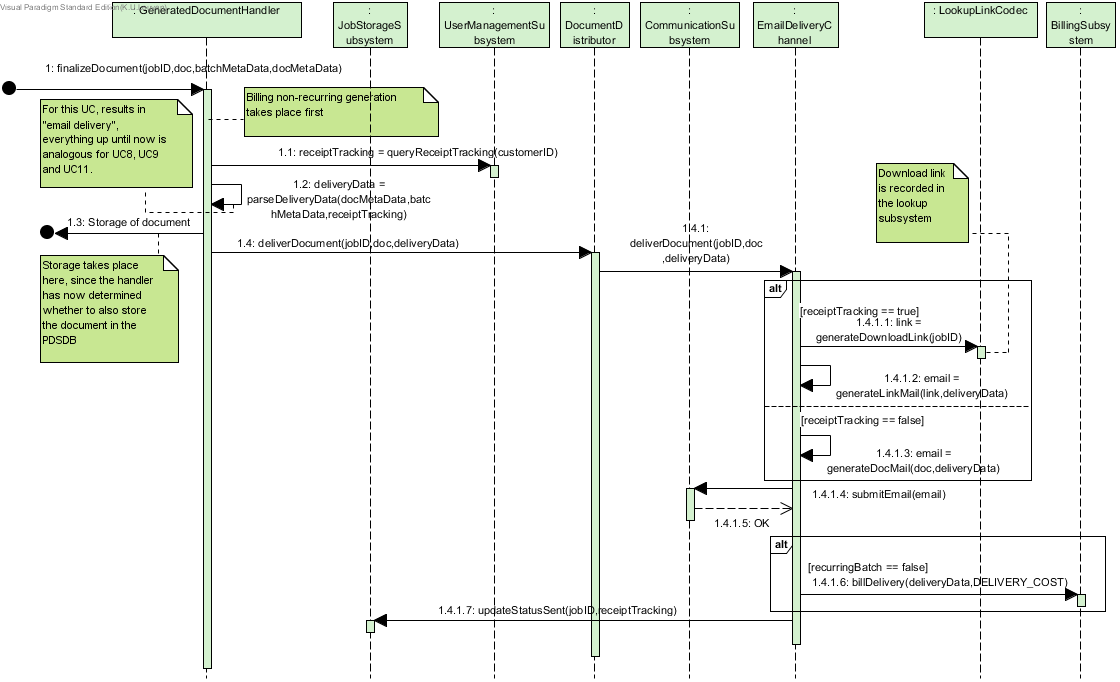
\includegraphics[width=\textwidth]{figures/UC6 - Deliver document via e-mail.png}
    %\missingfigure[figwidth=0.8\textwidth]{Sequence diagram scenario 1}
    \caption{The system behavior for the first scenario.
        }\label{fig:seq_scenario1}
\end{figure}